\section{Experiments and Evaluation}
We evaluate our method on KernelBench\cite{kernelbench}, a popular automated GPU program generation benchmark with 4 Levels. Levels 1 and 2 consist of kernel-level tasks: a single batched matrix multiplication kernel on Level 1 and a single Python file with Conv2D, ReLU, and BiasAdd on Level 2. Level 3 contains 50 end-to-end GPU programming tasks, such as a full VisionTransformer inference implementation with all kernel API calls (e.g., conv2d, relu, maxpool, attention). We identify limitations in KernelBench and address them through modifications; details are provided in Appendix~\ref{app:bench}.



The inputs are generated randomly in various numerical values and shapes for each task. All the reference PyTorch codes in KernelBench are run in eager mode without enabling \texttt{torch.compile}. For Level 3, we also provide an additional comparison with \texttt{torch.compile} enhanced reference code in the main result section. We do not apply it in the reference code for Level 1/2, given its minor impact on performance in single-kernel tasks.



We use Qwen3-32B \cite{qwen3technicalreport,hui2024qwen2} as our RL base model for Coder in our multi-agent framework and GPT-5.2 as the Planner and Verifier. 
 
We evaluate our method and baselines at KernelBench levels 1, 2, and 3 on 2 of the most advanced GPUs: the NVIDIA H200 (Hooper Architecture) and RTX PRO 6000 (Blackwell Architecture), separately. To fully evaluate the effectiveness of StitchCUDA, we apply various baselines as shown in Table~\ref{tab:l3}, including general and domain-specific LLMs, their performance as the Coder in our multi-agent framework, and the only open-source multi-agent framework, CUDAForge~\cite{cudaforge}, using GPT-5.2 as Coder and Judge.
We enable thinking for all LLMs in our experiments and evaluate all baselines and StitchCUDA with 15 iterations in 3 metrics: 
\vspace{-10pt}
\begin{itemize}
    \item \textit{Success Rate}, is measured by checking whether the generated code’s output falls within a predefined error tolerance of the reference implementation across multiple random seeds. A task is deemed successful if the tolerance is met in at least one iteration, independent of speedup. All successful cases are manually reviewed to filter out hacking results (e.g., PyTorch-only code). 
    \item \textit{E2E Average Speedup}, is computed as the ratio between the average end-to-end runtime(including data movement, kernel launch, CPU-GPU synchronization, and GPU kernel time) of the reference code and the generated code for each task. Following \cite{cudaforge}, the reported runtime for the generated code is the best result obtained over 15 refinement iterations.
    \item $\rm{Fast}_1$, A standard metric used in KerneBench ~\cite{kernelbench} that accounts for both success rate and achieved speedup, defined as: 
$\rm{Fast}_1=1/N \sum_{i=1}^{N}(correct_i\wedge{speedup_i > 1})$
   
    where N is the number of tasks.
    
\end{itemize}


\begin{table*}[h]
\caption{The success rate and E2E mean speedup relative to PyTorch Eager of various methods on our testing set. The best results are highlighted in \textbf{bold}, the second best is \underline{underline}. StitchCUDA-Q is our multi-agent framework, with the original Qwen3-32B as the Coder. Similarly, StitchCUDA-K is a backend with Kevin32B, StitchCUDA-G is a backend with GPT-5.2 as Coder, and StitchCUDA-C is a backend with Claude-4.6-Sonnet.}
\label{tab:l3}
{\fontsize{7}{8}\selectfont
\begin{tabular}{c|c|ccc|ccc|ccc}
\hline
                                                                                 &                                    & \multicolumn{3}{c|}{Level 1 (20 Tasks)}                       & \multicolumn{3}{c|}{Level 2 (20 Tasks)}                       & \multicolumn{3}{c}{Level 3 (10 Tasks)}                                                           \\ \cline{3-11} 
\multirow{-2}{*}{Hardware}                                                       & \multirow{-2}{*}{Method}           & Correctness    & Avg Speedup    & $\rm{Fast}_1$           & Correctness    & Avg Speedup    & $\rm{Fast}_1$ & Correctness                 & Avg Speedup                  & $\rm{Fast}_1$                   \\ \hline
                                                                                 & GPT5.2                             & 10/20          & 0.73x          & 25\%          & 8/20           & 0.66x          & 30\%             & 2/10                        & 0.47x                        & 10\%                     \\
                                                                                 & Claude-4-sonnet                    & 12/20          & 1.02x          & 25\%             & 8/20           & 0.76x          & 30\%             & 3/10                        & 0.67x                        & 20\%                     \\
                                                                                 & Qwen3-32B                          & 2/20           & 0.02x          & 5\%           & 0            & 0              & 0\%                & 0                           & 0                            & 0\%                     \\
                                                                                 & Kevin32B                           & 9/20           & 0.65x          & 10\%             & 11/20          & 0.49x          & 30\%             & 4/10                        & 0.22x                        & 0\%                        \\
                                                                                 & CUDAForge                          & {\underline{18/20}}    & 2.74x          & {\underline {50\%}}       & \underline{18/20}          & 1.28x          & 80\%             & 6/10                        & 0.75x                        & 30\%                     \\
                                                                                 & StitchCUDA-Q  
                                                                                 & 3/20 & 0.19x & 5\% & \underline{18/20}              & 0.77x              & 45\%                & 6/10	&0.40x	& 10\%                               \\
                                                                                 & \multicolumn{1}{l|}{StitchCUDA-K} & 13/20          & 2.11x          & 30\%          & 17/20          & 0.82x          & 65\%          & 7/10 & { 0.42x} & { 0\%} \\
                                                                                 & \multicolumn{1}{l|}{StitchCUDA-G} & \textbf{19/20} & \underline{3.97x} & \textbf{55\%} & \textbf{19/20} & \underline{1.87x} & \textbf{95\%} & 6/10                  & { 0.99x}                  & {\underline{ 50\%}}            \\
                                                                                 & StitchCUDA-C                            & \underline{18/20}          & \textbf{4.15x}          & \textbf{55\% }         & \textbf{19/20}           & \textbf{1.89x}          & 80\%             & \underline{9/10}                        & \underline{1.18x}                        & \underline{50\%}                     \\
                                                                                 
\multirow{-9}{*}{\begin{tabular}[c]{@{}c@{}}PRO 6000\\ (BlackWell)\end{tabular}} & StitchCUDA                        & {\underline{ 18/20}}    & {\ 2.86x}    & 35\%          & \textbf{19/20} & { 1.55x}   & {\underline{ 85\%}}    & \textbf{10/10}              & \textbf{1.27x}               & \textbf{70\%}            \\ \hline
                                                                                 & GPT5.2                             & 10/20          & 0.6x           & 20\%             & 9/20           & 0.63x          & 30\%             & 2/10                        & 0.48x                        & 10\%                     \\
                                                                                 & Claude-4-sonnet                    & 12/20          & 1.04x          & 30\%             & 10/20          & 0.78x          & 30\%             & 3/10                        & 0.64x                        & 20\%                     \\
                                                                                 & Qwen3-32B                          & 2/20           & 0.21x          & 5\%           & 0              & 0              & 0\%                & 0                           & 0                            & 0\%                        \\
                                                                                 & Kevin32B                           & 9/20           & 0.62x          & 10\%             & 10/20          & 0.53x          & 30\%             & 2/10                        & 0.34x                        & 10\%                        \\
                                                                                 & CUDAForge                          & \textbf{18/20} & 3.18x          & 45\%          & \underline{18/20}          & 1.43x          & 75\%          & 6/10                        & 0.87x                        & 40\%                  \\
                                                                                 & StitchCUDA-Q                      & \underline{17/20}          & 2.13x          & 20\%          & 16/20         & 0.94x          & 50\%          & 3/10                        & 0.24x                        & 10\%                  \\
                                                                                 & \multicolumn{1}{l|}{StitchCUDA-K} & 12/20          & 2.25x          & \underline{50\%}          & 15/20          & 0.77x          & 60\%          & 5/10                        & 0.32x                        & 0\%                        \\
                                                                                 & \multicolumn{1}{l|}{StitchCUDA-G} & \textbf{18/20} & \textbf{3.57x} & 45\%          & \textbf{19/20} & {\underline {1.79x}}    & \textbf{90\%} & {\underline{ 6/10}}                  & {\underline{ 1.01x}}                  & {\underline{ 50\%}}            \\
\multirow{-9}{*}{\begin{tabular}[c]{@{}c@{}}H200\\ (Hooper)\end{tabular}}        & StitchCUDA                        & {\textbf{ 18/20}}    & {\underline{ 3.54x}}    & \textbf{55\%} & \underline{18/20}          & \textbf{1.82x} & {\underline{ 85\%}}    & \textbf{9/10}               & \textbf{1.50x}               & \textbf{70\%}         \\ \hline
\end{tabular}}
\end{table*}

\vspace{-15pt}
\subsection{Main results}
During RL for Coder, we randomly selected 80\% of tasks from Levels 1/2/3 to collect training data. We evaluate our method and all baselines on the remaining 20\% of tasks as the test set. The experiment results are shown in Table~\ref{tab:l3}. Across both GPUs, the results support the following claims: 
\paragraph{Multi-agent orchestration substantially improves end-to-end correctness and makes speedups attainable.}

We first evaluate the contribution of multi-agent orchestration by holding the Coder model fixed and only changing the workflow from single-shot generation to StitchCUDA’s multi-agent framework.
Using Qwen3-32B as an example (our RL base model), single-shot generation performs poorly in the end-to-end setting: on H200, Qwen3-32B achieves only \textbf{2/20} correctness on Level~1 and no successful cases on Level~2/3. In contrast, StitchCUDA-Q (same Qwen3-32B as Coder, \emph{no RL}) increases Level~1 correctness to \textbf{17/20} with \textbf{2.13$\times$} mean speedup, and makes harder levels attainable (Level~2: \textbf{16/20} correctness; Level~3: \textbf{3/10} correctness).
A similar trend holds for a stronger domain-specific RL model: Kevin32B alone remains limited on Level~3 (RTX PRO 6000: \textbf{4/10}, \textbf{0.22$\times$}; H200: \textbf{2/10}, \textbf{0.34$\times$}), while placing Kevin32B into our multi-agent workflow (StitchCUDA-K) substantially improves correctness on harder benchmarks (RTX PRO 6000 Level~3: \textbf{4/10}$\rightarrow$\textbf{7/10};  H200 Level~3: 2/10 $\rightarrow$ 5/10). Even for advanced GPT-5.2 and Claude-4.6-Sonnet, the trend holds the same(GPT-5.2 v.s. StitchCUDA-G and Claude-4.6-Sonnet v.s. StitchCUDA-C).
These comparisons indicate that our multi-agent decomposition and tool-augmented iteration are essential, improving the performance of various models.

\paragraph{Agentic RL strengthens the multi-agent loop into consistent optimization on end-to-end tasks.}
We evaluate the impact of agentic RL by comparing StitchCUDA against its no-RL variant, StitchCUDA-Q. RL yields a dominant gain on the hardest Level~3 tasks. On H200 GPU, correctness improves from \textbf{3/10} to \textbf{9/10}, mean speedup increases from \textbf{0.24$\times$} to \textbf{1.50$\times$}, and $\rm{Fast}_1$ rises from \textbf{10\%} to \textbf{70\%}. The same pattern holds on Level~2 (from \textbf{16/20}, \textbf{0.94$\times$}, \textbf{50\%} $\rightarrow$ \textbf{18/20}, \textbf{1.82$\times$}, \textbf{85\%}) and Level~1 (same corrcetness with better speedup and $\rm{Fast}_1$). And this trend holds the same on RTX PRO 6000. This shows that our rubric-based agentic RL is the key factor driving significant real-system-level speedups, rather than merely improving correctness.
\paragraph{Agentic RL gains persist beyond using a stronger model.}
Even compared to StitchCUDA-G (GPT-5.2 as all agents), StitchCUDA achieves substantially stronger Level~3 results on both GPUs, with a much smaller 32B Coder model. StitchCUDA and StitchCUDA-G gain similar performance on Level~1/2, with nearly 100\% correctness and best or second-best mean speedup. On Level~3, StitchCUDA surpasses StitchCUDA-G on all metrics, and is the only method that can achieve nearly 100\% correctness on Level~3. 



We evaluate StitchCUDA, StitchCUDA-G, and Kevin-32B on the Level 3 test set with reference code enabling \texttt{torch.compile} on H200 GPU. Kevin32B achieves lower speedup from 0.34$\times$ in eager mode compared to 0.18$\times$ in \texttt{torch.compile} enabled reference code. StitchCUDA-G achieves 0.92$\times$ speedup, lower than its 1.01$\times$ in eager mode. StitchCUDA achieves 1.29$\times$, also lower than 1.50$\times$ in eager mode, but still better than the reference code. 
We want to emphasize that \textbf{our agents manually perform system optimization as a result of improvement over \texttt{torch.compile}, such as custom kernel fusion and data movement optimization, without introducing compiler overhead}.



\label{sec:main_result}
\subsection{Ablation Study}
To comprehensively evaluate the effect of the rubric reward, we conduct an ablation study. 
We introduce StitchCUDA-A, an ablated variant of StitchCUDA
trained with \emph{only} the rule-based reward (correctness and speedup; see
Appendix~\ref{kevinreward}) using Qwen3-32B. As shown in Fig~\ref{fig:ablation}, we evaluate StitchCUDA-A
on KernelBench Levels~1/2/3. Relative to StitchCUDA,
StitchCUDA-A achieves a comparable success rate on Levels~1/2, but a
lower success rate on Level~3 and lower speedup across Levels~1/2/3, indicating
that rubric reward is critical for effective RL training. We further inspect
Level~3 failures to understand the role of rubric reward and observe three
recurring patterns: \textbf{(1) Degenerate solutions.} The model often
produces overly conservative, low-performance implementations; \textbf{(2) Weak
feedback following.} Without explicit reward, the model’s ability to act on feedback degrades; and \textbf{(3) Reward hacking.} In the absence of reward penalties, the model exhibits reward hacking similar to Kevin-32B. Additional analysis for reward-hacking is provided in Section~\ref{sec:hack}.

We also conducted a per-dimension ablation study of the 4 aspects of our rubrics. We train four variants, each removing one rubric dimension while keeping the other three, and evaluated on KernelBench Level~3 on H200 GPU. 

As shown in Table~\ref{tab:rubric}. The results reveal that each dimension contributes distinctly. Removing Anti-Hacking has the most severe overall impact: correctness drops sharply (9.0 → 5.7), hacking instances nearly double (7.7 → 15.7), and speedup degrades to 0.75×. This indicates that without explicit anti-hacking reward, the model extensively exploits reward loopholes, producing solutions that are neither correct nor genuinely optimized. This dimension serves as the foundation of the entire rubric system. Removing CUDA Engineering maintains reasonable correctness (8.0) and low hacking (9.3), but reduces speedup from 1.50× to 1.18×, confirming that this dimension drives genuine optimization quality by encouraging advanced techniques such as tiling, tensor cores, and kernel fusion. Removing Operator Coverage shows a similar pattern with even lower speedup (1.08×), as the model reverts to optimizing only trivial operators while leaving core bottlenecks untouched. Removing Skill Compliance primarily affects correctness (9.0 → 7.3) while maintaining moderate speedup (1.33×), indicating that the model retains optimization capability but fails to follow task specifications and Verifier feedback precisely. All single-dimension ablations outperform StitchCUDA-A (no rubric), confirming that the remaining three dimensions still provide meaningful training signal.


\begin{table}
    \centering
    \caption{Ablation results of training rubrics}
{\fontsize{8}{8}\selectfont
    \begin{tabular}{|c|c|c|c|}
\hline
\textbf{Variant}      & \textbf{Corre. (/10)} & \textbf{Speedup} & \textbf{Hacking (/50)} \\ \hline
StitchCUDA            & 9.0                        & 1.50×            & 7.7                             \\
w/o Anti-Hacking      & 5.7                        & 0.75×            & 15.7                            \\
w/o CUDA Engineering  & 8.0                        & 1.18×            & 9.3                             \\
w/o Operator Coverage & 8.0                        & 1.08×            & 10.0                            \\
w/o Skill Compliance  & 7.3                        & 1.33×            & 8.7                             \\
StitchCUDA-A          & 5.0                        & 0.46×            & 16.3                            \\ \hline
\end{tabular}}
    \label{tab:rubric}
\end{table}

\subsection{Hacking detection}
\label{sec:hack}
In our evaluation, we observe serious hacking behaviour on RL-based Kevin-32B, including writing PyTorch-only code or hardcoding output. We try to address it by using prompt engineering and test if the problem can be solved. Specifically, we explicitly add the following to the prompts: “You must at least customize one kernel in your implementation, and do not copy the original PyTorch API. You cannot hardcode output.” However, the problem remains. To gain a comprehensive understanding, we examine hacking behavior across the evaluations of the following 4 methods: StitchCUDA-K, StitchCUDA-Q, StitchCUDA-A, and StitchCUDA. Therefore, we can examine how RL influences hacking behaviors and the impact of the rubric reward, including the hacking penalty. 
 

Hacking detection is performed on our test sets across Levels~1/2/3, and the results are shown in Table~\ref{tab:hack}. We count two kinds of hacking:  \textbf{partial hacking} and \textbf{total hacking}. The former means the model exhibits hacking behavior in the 15 rounds' iteration, while the latter means all 15 results exhibit hacking behavior. The hacking behavior is counted by CUDA experts, containing “PyTorch-only code” and “hardcode output”.

According to our results, even with explicit prompts, StitchCUDA-K using RL-based Kevin-32B exhibits 22 partial hackings in the whole test and gets 4 total hackings, significantly worse than StitchCUDA-Q with  Qwen3-32B. However, another RL-based StitchCUDA-A performs 10 partial hackings but do not exhibit any total hacking. We attribute it to  our RL trains the model to follow feedback, where we ask the model not to hack. In contrast, StitchCUDA performs the lowest hacking rate (8 partial hackings) in the test, demonstrating the effectiveness of rubric reward for anti-hacking.

\begin{figure}[t]
    \centering
    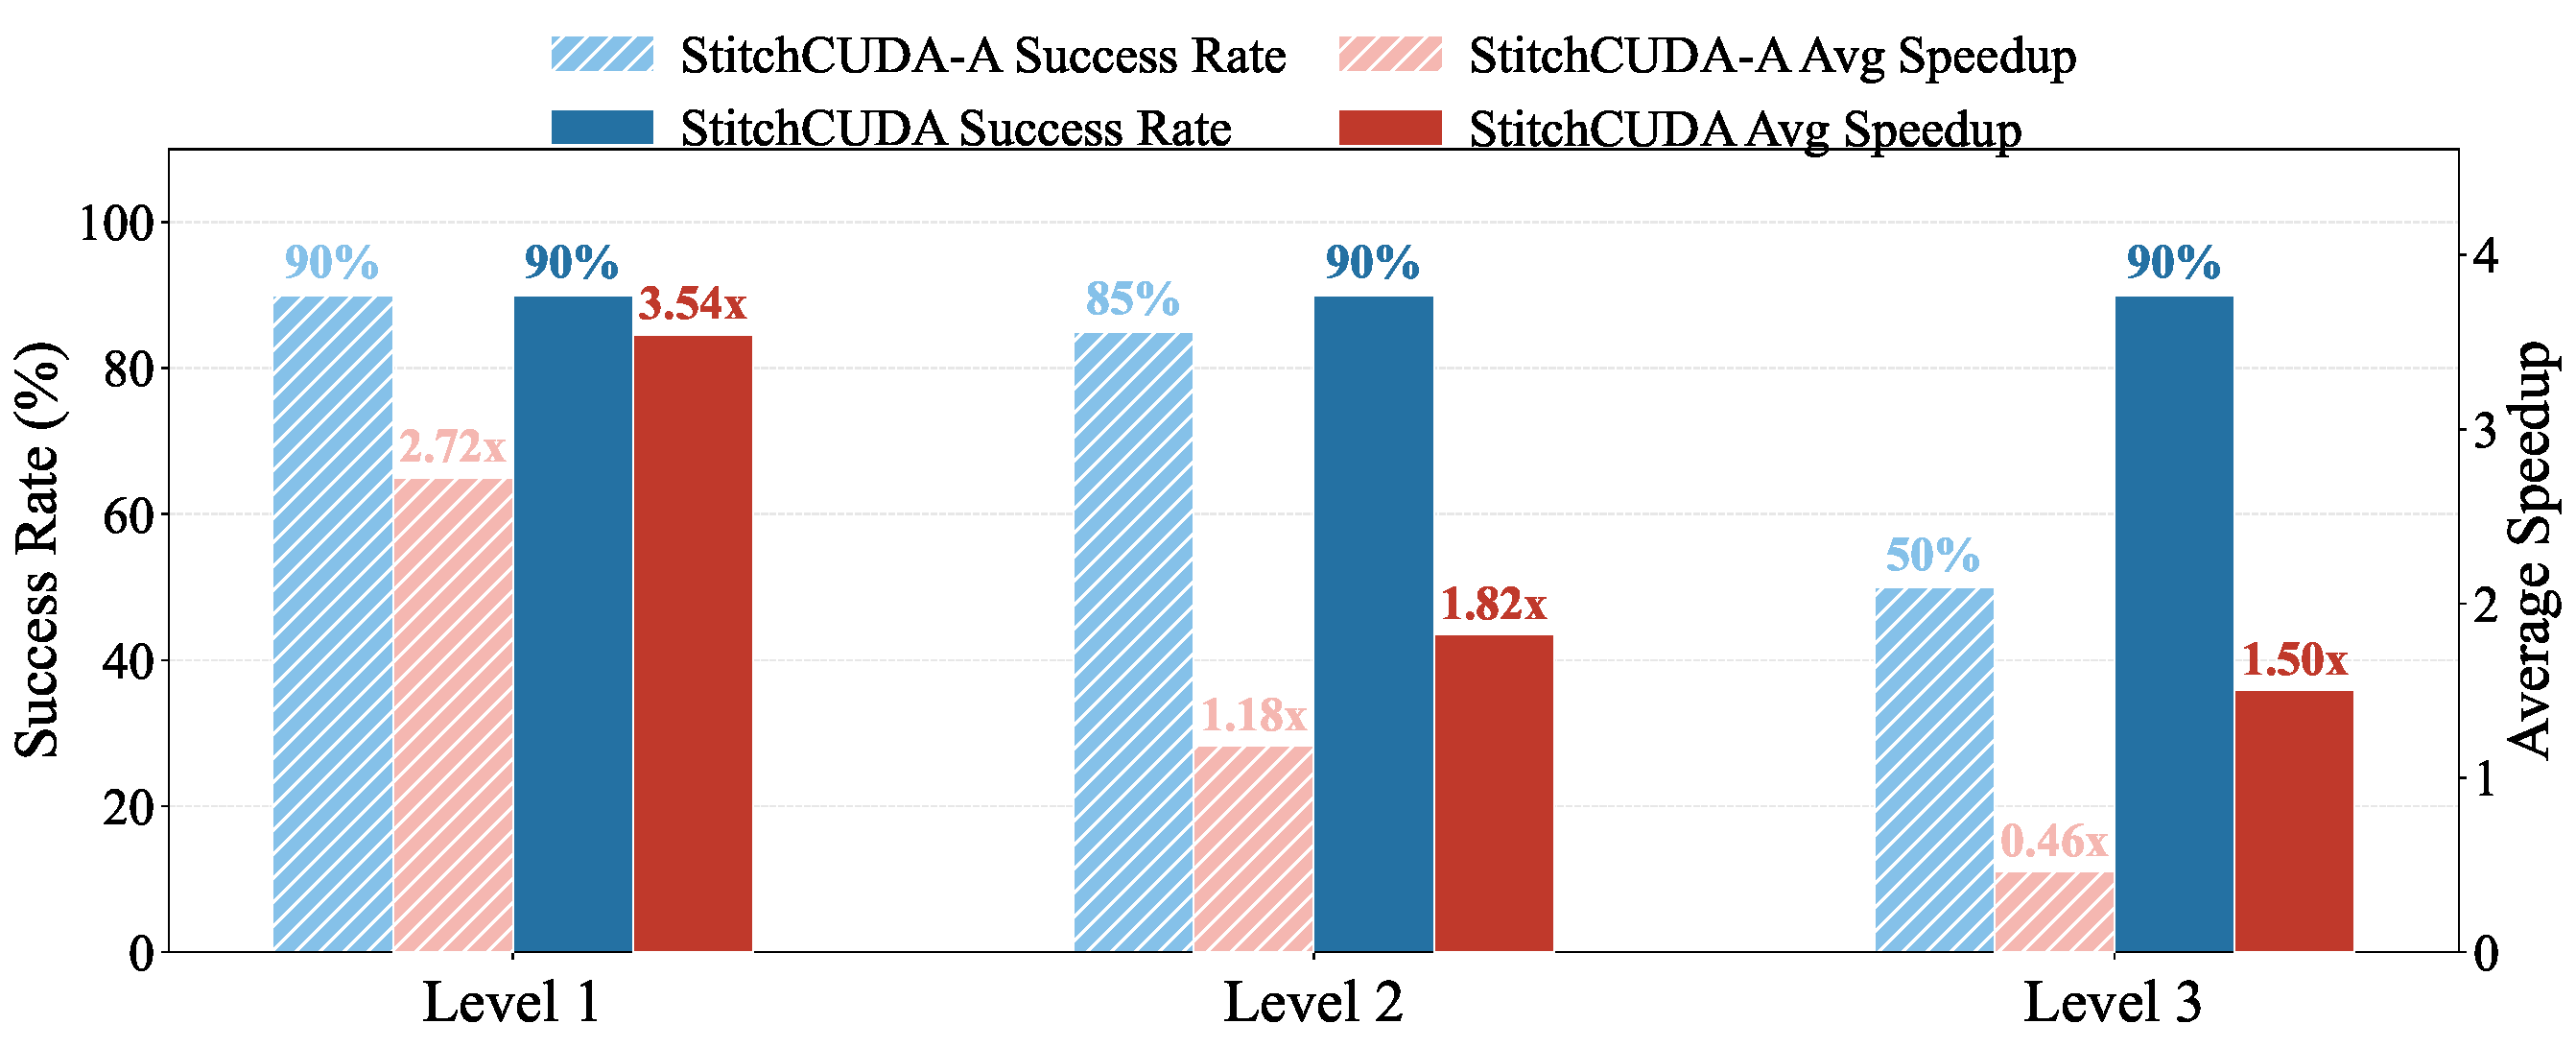
\includegraphics[width=\linewidth]{pic/ablation_graph.pdf}
    \caption{Comparison of success rate and average speedup between StitchCUDA and StitchCUDA-A across Level 1/2/3. StitchCUDA
  achieves higher success rates and speedups at all levels, with the rubric-based reward.}
    \label{fig:ablation}
    \vspace{-10pt}
\end{figure}


% Requires: \usepackage{multirow}
\begin{table}[h]
    \centering
    \tiny
    \caption{Hacking detection with prompts hint.}
    \label{tab:hack}
    {\fontsize{6}{7}\selectfont
    \begin{tabular}{l|cccccccc}
        \hline
        & \multicolumn{2}{c}{Level 1} & \multicolumn{2}{c}{Level 2} & \multicolumn{2}{c}{Level 3} & \multicolumn{2}{c}{Sum} \\
        \cline{2-9}
         Model& partial & total & partial & total & partial & total & partial & total \\
        \hline
        StitchCUDA-K     & 10 & 3 & 8 & 0 & 4 & 1 & 22/50 & 4/50 \\
        StitchCUDA-Q     & 4  & 0 & 4 & 0 & 2 & 0 & 10/50 & 0   \\
        StitchCUDA-A & 8  & 0 & 5 & 0 & 3 & 0 & 16/50 & 0   \\
        StitchCUDA & 3  & 0 & 3 & 0 & 2 & 0 & 8/50  & 0   \\
        \hline
    \end{tabular}}
\end{table}


